\documentclass{article}

% Packages
\usepackage[utf8]{inputenc} % For modern characters
\usepackage{microtype} % For sexy kerning
\usepackage{mathtools} % For math stuff
\usepackage{amssymb} % For math symbols
\usepackage{tabularx} % For making tables
\usepackage{fancyhdr} % Use a header
%\usepackage{fullpage} % Get rid of white space in margins
% fullpage package doesn't work with fancyhdr

% Set the margins
\usepackage[scale=0.8, top=1in, bottom=1in]{geometry}

% Other front matter
\newcommand{\code}[1]{\texttt{#1}} % More readable for writing inline code.
\newcommand{\p}[1]{\paragraph{#1}} % Easier to type out for paragraph command
\newcommand{\addsection}[1]{\addcontentsline{toc}{section}{#1}} % content lines
\newcommand{\addsubsection}[1]{\addcontentsline{toc}{subsection}{#1}} % content lines
\pagestyle{fancy} % Makes Header Possible
{ %%% Header Set up
	\lhead{} % Set the left header to be blank
	\chead{} % Set the center header to be blank
	% Header for every page except the first two
	\rhead{Ben Foster | Homework 4 | May 8, 2015} % Name, assignment, date
}
\setcounter{tocdepth}{2} % Set Table of Contents Depth
\setlength{\parindent}{0pt} % Disable automatic indentation

%%%%%%%%%%%%%%%%%%%%% Begin Document %%%%%%%%%%%%%%%%%%%%%
\begin{document}

{ % Title page, table of contents, and page number setting
	\title{Probability and Statistics for Engineers Homework Four \\ TMATH 390}
	\author{Ben Foster\thanks{
		Institute of Technology, University of Washington Tacoma} \\
		Instructor: Julia Eaton}
	\date{May 8, 2015}
	\maketitle
	\thispagestyle{empty} % No page number at bottom
	\clearpage
	
	\pagenumbering{roman}
	\tableofcontents
	\clearpage
	\setcounter{page}{1}
	\pagenumbering{arabic}
}

\p{Chapter 3 questions:} all but one should be done in R. 

\section*{Problem 1} %%% DONE
\addsection{First Problem}

	\textbf{(Interpreting output from statistical software)} Here is a relatively standard-looking output 
	from some statistical software. The data deals with predicting concrete strength from its 
	modulus of elasticity. \\

	\begin{tabular}{ l l l l l }
		Predictor & Coeff & Stdev & t-ratio & p \\
		Constant & 3.2925 & 0.6008 & 5.48  & 0.000 \\
		mod elas & 0.10748 & 0.01280 & 8.40 & 0.000 \\
	\end{tabular} \\
	\begin{tabular}{ c c c }
		s = 0.8657 & R-sq = 73.8\% & R-sq (adj) = 72.8\%
	\end{tabular} \\
	
	Analysis of Variance: \\
	\begin{tabular}{ l l l l l l }
		SOURCE & DF & SS & MS & F & p \\
		Regression & 1 & 52.870 & 52.870 & 70.55 & 0.000 \\
		Error & 25 & 18.736 & 0.749 & & \\ 
		Total & 26 & 71.605 & & &
	\end{tabular} \\
	
	User your knowledge of regression and the various quantities that arise within regression to: \\
	(a) Identify the estimated intercept and slope in the regression equation, and interpret them. \\
	(b) Identify $SS_{total}$, $SS_{explained}$, and $SS_{unexplained}$. \\
	(c) Identify $R^2$ and state what it means (it is a percentage of...). \\
	
	\addsubsection{Answer to 1.a}
	\p{Answer to a}
	From looking at the given data, the slope is $\alpha = 0.10748$ and the intercept is $\beta = 
	3.2925$. This shows that the line with closest fit doesn't have a very large slope and seems 
	almost uniform.
	\[ \hat{y} = 3.2925 + 0.10748(x) \]
	
	\addsubsection{Answer to 1.b}
	\p{Answer to b}
	In order to find $SS_{total}$, $SS_{explained}$, and $SS_{unexplained}$, all we have to do is 
	look at the given data. \\
	$SS_{explained} = 52.870$\\
	$SS_{unexplained} = 18.736$ \\
	$SS_{total} = 71.605$.
	
	\addsubsection{Answer to 1.c}
	\p{Answer to c}
	From looking at the given data, $R^2 = 73.8\%$ or 0.738. This is a percentage of how well the 
	regression line approximates the actual data points given.

\clearpage
\section*{Problem 2} %%% DONE
\addsection{Second Problem}

	\textbf{(Transforming data)} The article "Reduction in Soluble Protein and Chlorophyll Contents 
	in a Few Plants as Indicators of Automobile Exhaust Pollution" (Intl. J. of Environ. Studies, 
	1983: 239-244) reported the accompanying data on $x$ distance from a highway (meters) and 
	$y$ lead content of soil at a distance (parts per million, or ppm):
	
	\begin{center}
	\begin{tabular}{ l l l l l l l l l l l l l }
		$x$: & 0.3 & 1 & 5 & 10 & 15 & 20 & 25 & 30 & 40 & 50 & 75 & 100 \\
		$y$: & 62.75 & 37.15 & 29.70 & 20.71 & 17.65 & 15.41 & 14.15 & 13.50 & 12.11 & 11.40 & 
		10.85 & 10.85 \\
	\end{tabular}
	\end{center}
	
	(a) Construct scatter plots of $y$ versus $x$, $y$ versus $ln(x)$, $ln(y)$ versus $ln(x)$, and $
	\frac{1}{y}$ versus $\frac{1}{x}$. \\
	(b) Based on the results of part (a), which transformation does the best job of producing an 
	approximate linear relationship? \\
	(c) Use the selected transformation to predict lead content when distance is 45 meters. \\
	
	\addsubsection{Answer to 2.a}
	\p{Answer to a}\mbox{}\\
	
	\addsubsection{Graph of $y$ versus $x$}
	\p{Graph of $y$ versus $x$}
	\begin{center}
		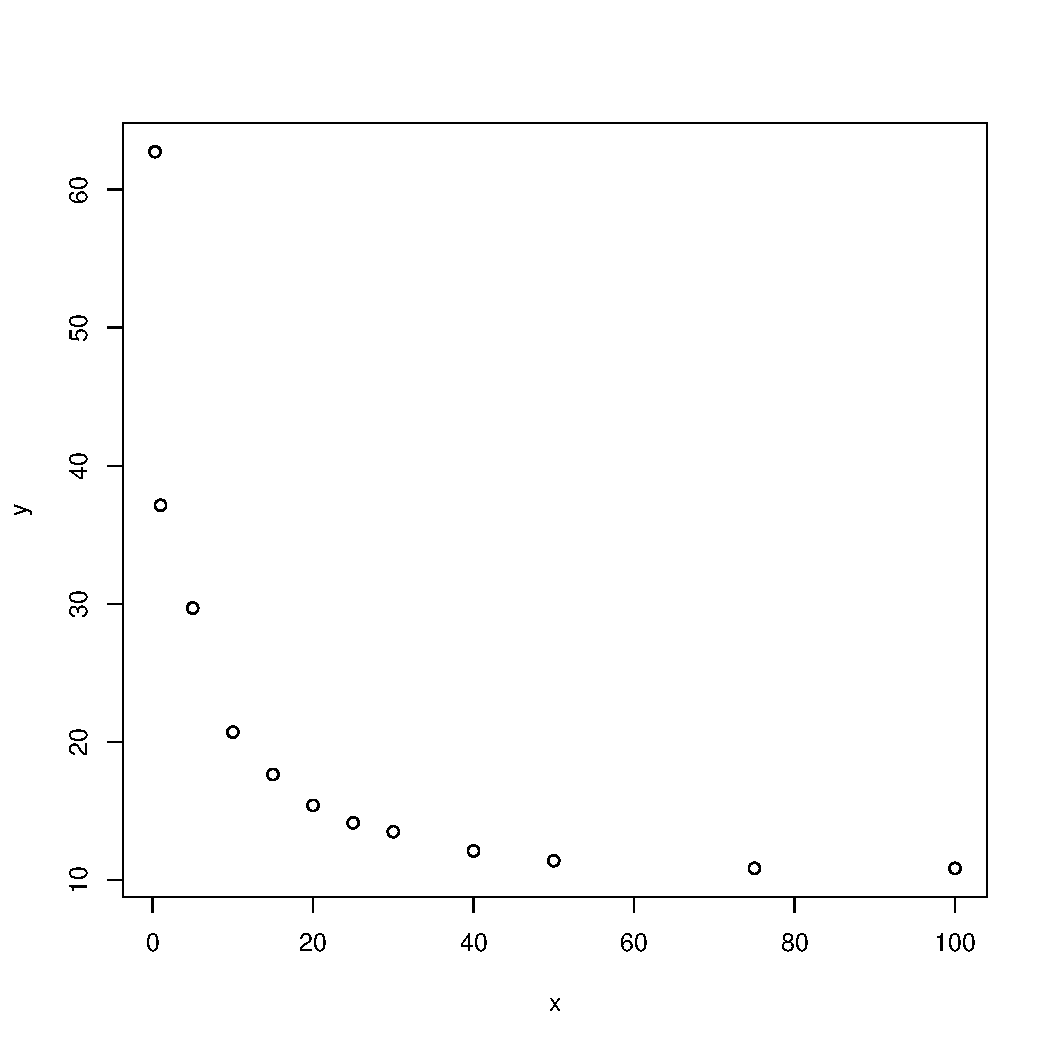
\includegraphics[width=4in]{img/Hwk4_prob2_1.pdf}
	\end{center}
	
	\clearpage
	\addsubsection{Graph of $y$ versus $ln(x)$}
	\p{Graph of $y$ versus $ln(x)$}
	\begin{center}
		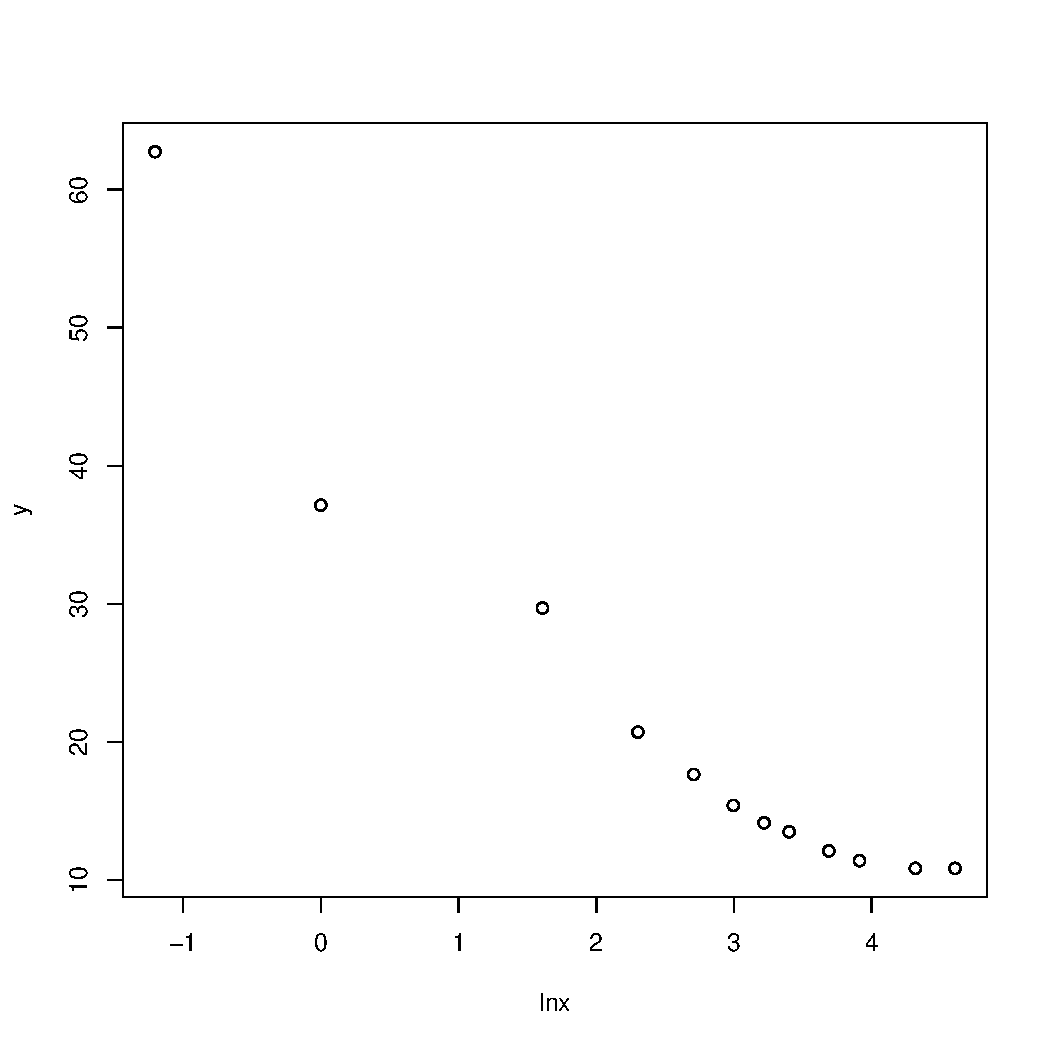
\includegraphics[width=4in]{img/Hwk4_prob2_2.pdf}
	\end{center}
	
	\addsubsection{Graph of $ln(y)$ versus $ln(x)$}
	\p{Graph of $ln(y)$ versus $ln(x)$}
	\begin{center}
		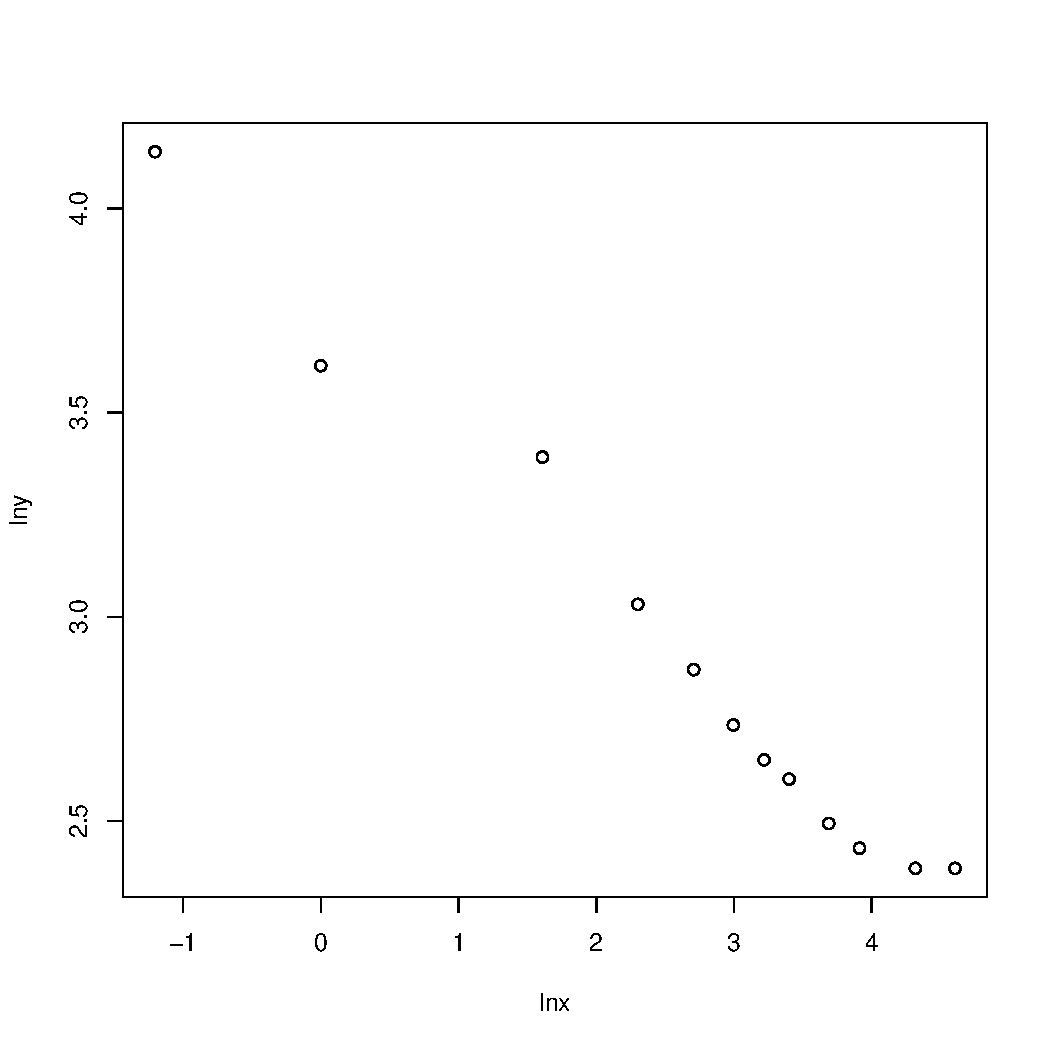
\includegraphics[width=4in]{img/Hwk4_prob2_3.pdf}
	\end{center}
	
	\clearpage
	\addsubsection{Graph of $\frac{1}{y}$ versus $\frac{1}{x}$}
	\p{Graph of $\frac{1}{y}$ versus $\frac{1}{x}$}
	\begin{center}
		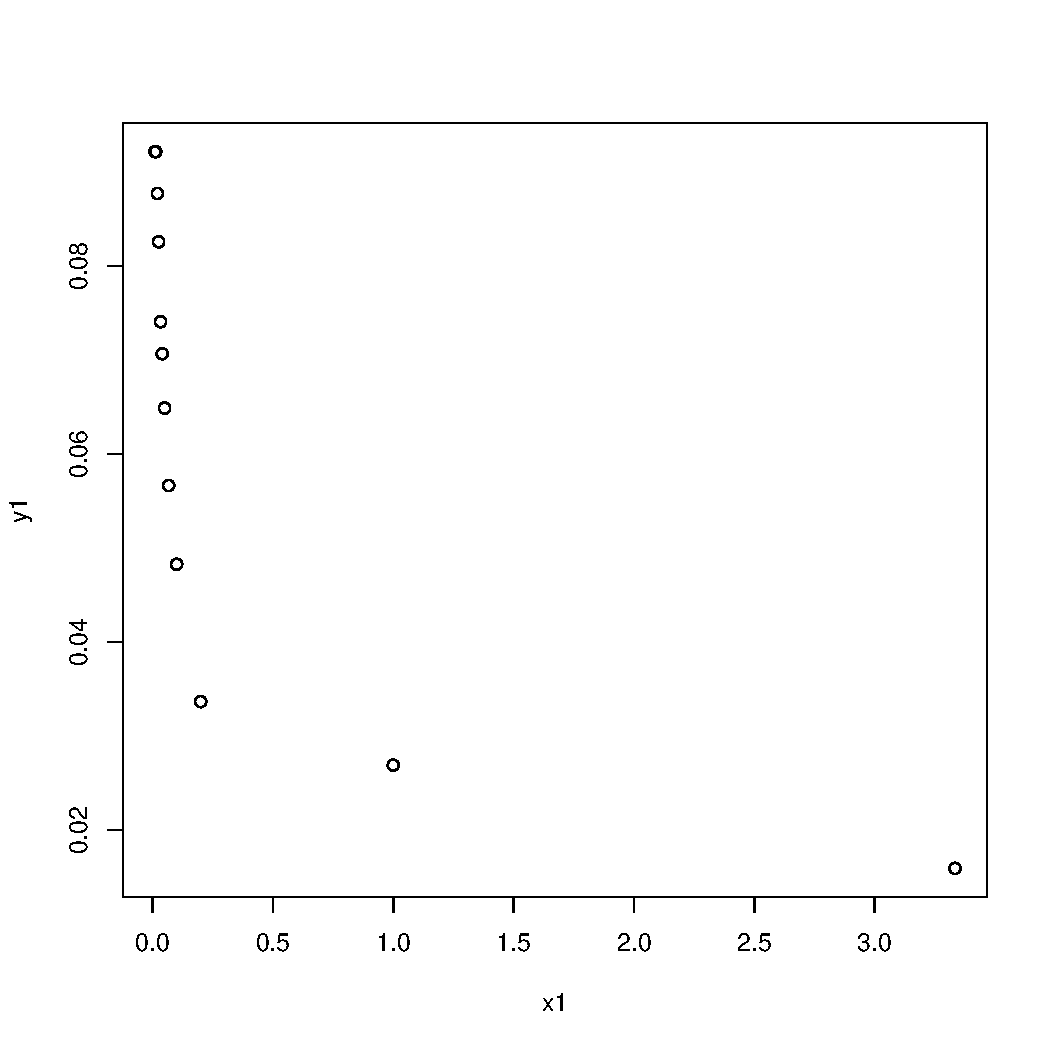
\includegraphics[width=4in]{img/Hwk4_prob2_4.pdf}
	\end{center}
	
	\addsubsection{Answer to 2.b}
	\p{Answer to b}
	Based on the results of part(a), the transformation that does the best job of producing an 
	approximate linear relationship is the transformation $ln(y)$ versus $ln(x)$.
	
	\addsubsection{Answer to 2.c}
	\p{Answer to c}
	Using the selected transformation, when the distance is 45 meters, the corresponding lead 
	content will be about 12.46 ppm.
	
	\[ ln(\hat{y}) = 3.72433 - (0.3157)ln(x) \]
	\[ \hat{y} = e^{2.523} \]
	\[ \hat{y} = 12.461 \]

\clearpage
\section*{Problem 3} %%% DONE
\addsection{Third Problem}

	\textbf{(Polynomial regression)} One frequently encountered problem in crop production is deciding when to harvest to maximize yield. Data on the time to harvesting (number of days after flowering) and the yield (kg/ha) of paddy|a grain farmed in India|appeared in the article "Determination of Biological Maturity and Effect of Harvesting and Drying Conditions on Milling Quality of Paddy" (J. of Agric. Engr., 1975: 353-361), and appears below. \\
	
	\begin{tabular}{ l l l l l l l l l }
		(time to harvest): & 16 & 18 & 20 & 22 & 24 & 26 & 28 & 30 \\
		(paddy yield): & 2508 & 2518 & 3304 & 3423 & 3057 & 3190 & 3500 & 3883
	\end{tabular} \\
	
	\begin{tabular}{ l l l l l l l l l }
		(time to harvest): & 32 & 34 & 36 & 38 & 40 & 42 & 44 & 46 \\
		(paddy yield): & 3823 & 3646 & 3708 & 3333 & 3517 & 3241 & 3103 & 2776
	\end{tabular} \\
	
	(a) Is it possible to transform this data as described in this section so that there is an 
	approximate linear relationship between the transformed variables? Why or why not? (Think 
	about the goal of the researchers: to maximize yield.) \\
	(b) Use a statistical computer package to fit a quadratic function to this data, and then predict 
	yield when time to harvesting is 25 days. Asses the fit of the quadratic data, i.e., interpret the 
	$R^2$ and the standard deviation about regression, $s_e$. Remember if you want to do 
	quadratic regression of $y$ versus $x$ you should use this: 
	\code{lm( y $\sim$ x + I(x\textasciicircum 2))} in R.
	
	\addsubsection{Answer to 3.a}
	\p{Answer to a}
	The data appears to fit a quadratic relationship more and therefore it is not possible to transform 
	the given data to approximate a linear relationship.
	
	\addsubsection{Answer to 3.b}
	\p{Answer to b}
	Using the code above and the command \code{summary(lm$\sim$x + I(x\textasciicircum2))}, we 
	get the following data: \\
	
	Residuals:
	\begin{tabular}{ c c c c c }
		Min & 1Q & Median & 3Q & Max \\
		-303.96 & -118.11 & 13.86 & 115.67 & 319.06 \\
	\end{tabular} \\
	
	\begin{tabular}{ l r r r r }
		Coefficients: & Estimate & Std. Error & t value & Pr(\textless$|t|$) \\
		(Intercept) & -1070.3977 & 617.2527 & -1.734 & 0.107 \\
		x & 293.4829 & 42.1776 & 6.958 & 9.94e-06 \\
		I(x\textasciicircum2) & -4.5358 & 0.6744 & -6.726 & 1.41e-05 \\
	\end{tabular} \\
	
	Residual standard error: 203.9 on 13 degrees of freedom \\
	Multiple R-squared: 0.7942, Adjusted R-squared: 0.7625 \\
	F-statistic: 25.08 on 2 and 13 DDF, p-value: 3.452e-05 \\
	
	From the data, we can see that $R^2 = 0.7942$ and $s_e = 203.9$. This means that the 
	regression line determined has about an 80\% fit. This is pretty good. We are also able to grab 
	the equation:
	\[ \hat{y} = -(4.5358)x^2 + (293.4829)x - 1070.3977 \]
	We can then use this formula to predict the yield when time to harvesting is 25 days:
	\[ \hat{y} = -(4.5358)(25)^2 + (293.4829)(25) - 1070.3977 \]
	\[ \hat{y} =  -2834.875 + 7337.0725 - 1070.3977 \]
	\[ \hat{y} = 3431.7998 \]
		
	\clearpage
	\addsubsection{Graph of data with line fit}
	\p{Graph of data with quadratic line fit}
	\begin{center}
		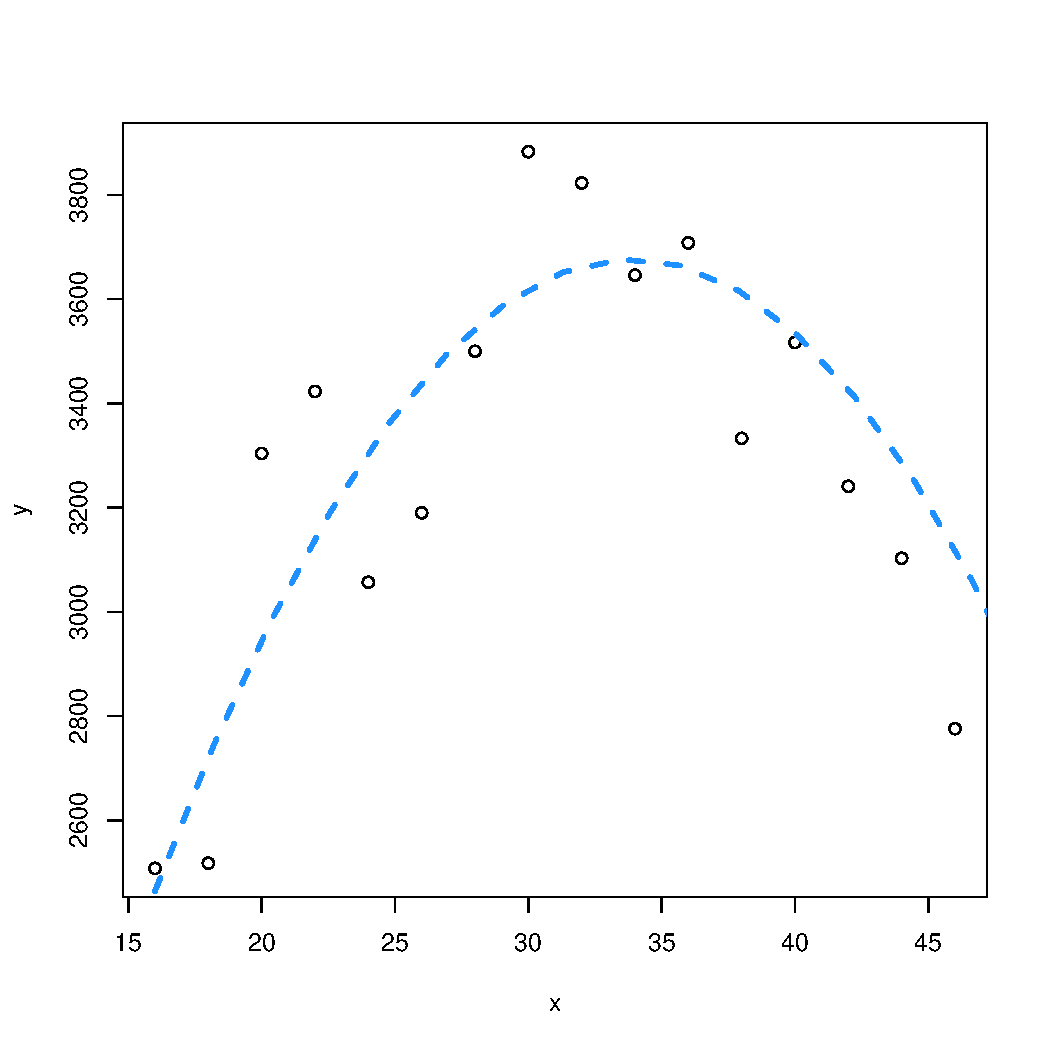
\includegraphics[width=\textwidth]{img/Hwk4_prob3.pdf}
	\end{center}

\clearpage
\section*{Problem 4} %%% DONE
\addsection{Fourth Problem}

	\textbf{(Polynomial regression two independent variables)} The article "The Undrained Strength of 
	Some Thawed Permafrost Soils" (Canadian Geotech. J., 1979: 420-427) contained the 
	accompanying data on $y$ shear strength of sandy soil (kPa), $x_1$ depth (m), and $x_2$ water 
	content (\%).
	
	\begin{tabular}{ l l l l }
		Obs & Depth & Water & Strength \\
		1   & 8.9   & 31.5 & 14.7 \\
		2   & 36.6 & 27.0 & 48.0 \\
		3   & 36.8 & 25.9 & 25.6 \\
		4   & 6.1   & 39.1 & 10.0 \\
		5   & 6.9   & 39.2 & 16.9 \\
		6   & 6.9   & 38.3 & 16.8 \\
		7   & 7.3   & 33.9 & 20.7 \\
		8   & 8.4   & 33.8 & 38.8 \\
		9   & 6.5   & 27.9 & 16.9 \\
		10 & 8.0   & 33.1 & 27.0 \\
		11 & 4.5   & 26.3 & 16.0 \\
		12 & 9.9   & 37.0 & 24.9 \\
		13 & 2.9   & 34.6 & 7.3 \\
		14 & 2.0   & 36.4 & 12.8
	\end{tabular}
	
	(a) Perform regression to predict $y$ from $x_1, x_2, x_1^2, x_2^2$. Remember to put $I()$ 
	around any terms you're squaring. You don't need it around "\code{x1 * x2}". Write down the 
	coefficients of the various terms. \\
	(b) Compute the $R^2$ and explain what it says about goodness-of-fit. \\
	(c) Now perform regression to predict $y$ from $x_1$ and $x_2$ only. \\
	(d) Compute $R^2$ and explain what it says about goodness-of-fit. \\
	(e) Compare the above two $R^2$ values. Does the comparison suggest that at least one of the 
	higher order terms in the regression equation provides useful information about strength? \\
	
	Note: the data for this problem are posted. Below is code that loads the file.\\

	\code{dat = read.table("Hwk4\_prob\_4.dat", sep="\&", header=T)} \\
	\code{y = dat\$Strength} \\
	\code{x1 = dat\$Depth} \\
	\code{x2 = dat\$Water}
	
	\addsubsection{Answer to 4.a}
	\p{Answer to a}
	Using the command \code{summary(lm(y$\sim$ x1 + x2 + I(x1\textasciicircum 2) + 
	I(x2\textasciicircum 2) + I(x1 * x2))} we get the following table: \\
	\begin{tabular}{ r l l l l }
		Coefficients: & Estimate & Std. Error & t value & Pr(\textless$|t|$) \\
		(Intercept) & -140.22976 & 136.13743 & -1.030 & 0.3331 \\
		x1 & -16.47521 & 9.07116 & -1.816 & 0.1069 \\
		x2 & 12.82710 & 8.25854 & 1.553 & 0.1590 \\
		x1\textasciicircum 2 & 0.09555 & 0.07206 & 1.326 & 0.2214 \\
		x2 \textasciicircum 2 & -0.24339 & 0.12744 & -1.910 & 0.0925 \\
		x1 * x2 & 0.49864 & 0.23543 & 2.118 & 0.0670
	\end{tabular} \\
	
	From this table, we get the coefficients:
	\begin{tabular}{ c c c c c c }
		(Intercept) & x1 & x2 & I(x1\textasciicircum 2) & I(x2\textasciicircum 2) & x1 * x2 \\
		-140.22976 & -16.47521 & 12.82710 & 0.09555 & -0.24339 & 0.49864
	\end{tabular} \\
	
	Therefore:
	\[ \hat{y} = -140.23 - 16.48x_1 + 12.83x_2 + 0.096x_1^2 - 0.243x_2^2 + 0.499(x_1)(x_2) \]
	
	\clearpage
	\addsubsection{Answer to 4.b}
	\p{Answer to b}
	From the same command as above, we also get the following data: \\
	Residual standard error: 7.023 on 8 degrees of freedom \\
	Multiple R-squared: 0.7561, Adjusted R-squared: 0.6037 \\
	F-statistic: 4.961 on 5 and 8 DF, p-value: 0.02307 \\
	
	So from this we get $R^2 = 0.7561$. This means that 75.61\% of variability in strength can be 
	attributed to variation in depth and water content.
	
	\addsubsection{Answer to 4.c}
	\p{Answer to c}
	By typing in code similar to above: \code{summary(lm(y$\sim$ x1 + x2))}, we can get the 
	coefficients for predicting $y$ from $x_1$ and $x_2$: \\
	\begin{tabular}{ l r r r r }
		Coefficients: & Estimate & Std. Error & t value & Pr(\textless$|t|$) \\
		(Intercept) & 14.8893 & 23.2447 & 0.641 & 0.5349 \\
		x1 & 0.6607 & 0.2737 & 2.414 & 0.0344 \\
		x2 & -0.0284 & 0.6423 & -0.044 & 0.9655
	\end{tabular}\\
	
	From this table, we get the coefficients:
	\begin{tabular}{ c c c }
		(Intercept) & x1 & x2 \\
		14.8893 & 0.6607 & -0.0284
	\end{tabular} \\
	
	Therefore:
	\[ \hat{y} = 14.89 + 0.66x_1 - 0.028x_2 \]
	
	\addsubsection{Answer to 4.d}
	\p{Answer to d}
	From the previous command, we get the following data:\\
	Residual standard error: 9.019 on 11 degrees of freedom \\
	Multiple R-squared 0.447, Adjusted R-squared: 0.3465\\
	F-statistic: 4.446 on 2 and 11 DF, p-value: 0.03845 \\
	
	So from this we get $R^2 = 0.447$. This shows that this way of determining $y$ only from $x_1$ 
	and $x_2$ is not a very good way of predicting $y$. It's goodness of fit isn't very good.
	
	\addsubsection{Answer to 4.e}
	\p{Answer to e}
	Comparing the two $R^2$ values above, (0.7561 and 0.4470), we can see that determining $y$ 
	from more predictors is more accurate. So, yes, at least one of the higher order terms in the 
	regression equation provides useful information about strength.

\clearpage
\section*{Problem 5} %%% DONE
\addsection{Fifth Problem}

	\textbf{(Interpreting more output)} An experiment carried out to study the effect of the mole 
	contents of cobalt ($x_1$) and the calcination temperature ($x_2$) on the surface area of an iron 
	cobalt hydroxide catalyst ($y$) resulted in the following data ("Structural Changes and Surface 
	Properties of CoxFe3xO4 Spinels," J. of Chemical Tech. and Biotech., 1994: 161-170):
	
	\begin{tabular}{ l l l l l l l l l l l }
		$x_1$: & 0.6   & 0.6   & 0.6   & 0.6   & 0.6   & 1.0     & 1.0     & 1.0   & 1.0   & 1.0 \\
		$x_2$: & 200  & 250  & 400  & 500  & 600  & 200    & 250    & 400  & 500  & 600 \\
		$y$:     & 90.6 & 82.7 & 58.7 & 43.2 & 25.0 & 127.1 & 112.3 & 19.6 & 17.8 & 9.1
	\end{tabular} \\
	\mbox{} \\
	
	\begin{tabular}{ l l l l l l l l l l l }
		$x_1$: & 2.6 & 2.6 & 2.6 & 2.6 & 2.6 & 2.8 & 2.8 & 2.8 & 2.8 & 2.8 \\
		$x_2$: & 200 & 250 & 400 & 500 & 600 & 200 & 250 & 400 & 500 & 600 \\
		$y$: & 53.1 & 53.0 & 43.4 & 42.4 & 31.6 & 40.9 & 37.9 & 27.5 & 27.3 & 19.0 
	\end{tabular} \\
	
	A request to the SAS package to fit $\alpha + \beta_1x_1 + \beta_2x_2 + \beta_3x_1x_2$ 
	yielded the following output: \\
	
	Dependent Variable: SURFAREA \\
	
	Analysis of Variance: \\
	\begin{tabular}{ l r r r r r }
		Souce & DF & Sum of Squares & Mean Square & F Value & Prob \textgreater F \\
		Model & 3 & 15223.52829 & 5074.50943 & 18.924 & 0.0001 \\
		Error & 16 & 4290.53971 & 268.15873 & & \\
		Total & 19 & 19514.06800 & & &
	\end{tabular} \\
	\begin{tabular}{ l r }
		Root MSE 16.47555 & R-Square 0.7801 \\
		Dep Mean 48.06000 & Adj R-sq 0.7389 \\
		C.V 34.07314 & 
	\end{tabular}

	Parameter Estimates: \\
	\begin{tabular}{ l c r r r r }
		Variable & DF & Parameter Estimate & Standard Error & T & Prob \textless $|$T$|$ \\
		INTERCEP & 1 & 185.486740 & 21.19747682 & 8.750 & 0.0001 \\
		COBCON & 1 & -45.969466 & 10.61201173 & -4.332 & 0.0005 \\
		TEMP & 1 & -0.301503 & 0.05074421 & -5.942 & 0.0001 \\
		CONTEMP & 1 & 0.088801 & 0.02540388 & 3.496 & 0.0030
	\end{tabular} \\

	(a) Interpret the value of the coefficient of determination $R^2$. \\
	(b) Predict the value of surface area when cobalt content is 2.6 and temperature is 250. \\
	(c) Since $\beta_1$ is about -46.0, is it legitimate to conclude that if cobalt content increases by 
	1 unit while the values of the other predictors remain fixed, surface area can be expected to 
	decrease by 46 units? Explain your reasoning. \\

	\addsubsection{Answer to 5.a}
	\p{Answer to a}
	From the data provided above, we have a $R^2$ value of 0.7801. This means that 78.01\% of the 
	variance in $y$ can be explained by the equation for $\hat{y}$ shown above.

	\addsubsection{Answer to 5.b}
	\p{Answer to b}
	Using the following equation:
	\[ \hat{y} = 185.49 - 45.97x_1 - 0.302x_2 + 0.0888(x_1)(x_2) \]
	Then we can predict what the value of surface area will be when the cobalt content is 2.6 (x1) 
	and the temperature is 250 (x2).
	\[ \hat{y} = 185.49 - 45.97(2.6) - 0.302(250) + 0.0888(2.6)(250) \]
	\[ \hat{y} = 48.311\text{ units}^2 \]
	
	\addsubsection{Answer to 5.c}
	\p{Answer to c}
	No because the cobalt content predictor is present in more than one term of the polynomial. 
	Since the coefficient $\beta_3$ is also being multiplied by cobalt content while the other predictor 
	remains the same, then our final value will be altered by more or less than 46 units. If $\beta_3$ 
	were zero or if the cobalt content predictor only showed up in one term, then this would be true.

\end{document}